%**************************************************************************
%*
%*  Instrucciones para la platilla del informe final
%*
%*  
%*
%*  Filename: platillapaper.tex
%*
%*
%*  
%*  
%*
%**************************************************************************


\documentclass{wscpaperproc}
\usepackage[spanish]{babel}
\usepackage{latexsym}
\usepackage{graphicx}
\usepackage{mathptmx}
\usepackage[T1]{fontenc}
\usepackage{listings}

%****************************************************************************
% AUTHOR: You may want to use some of these packages. (Optional)
\usepackage{amsmath}
\usepackage{amsfonts}
\usepackage{amssymb}
\usepackage{amsbsy}
\usepackage{amsthm}
%****************************************************************************


%
%****************************************************************************
% AUTHOR: If you do not wish to use hyperlinks, then just comment
% out the hyperref usepackage commands below.

%% This version of the command is used if you use pdflatex. In this case you
%% cannot use ps or eps files for graphics, but pdf, jpeg, png etc are fine.

\usepackage[colorlinks=true,urlcolor=blue,citecolor=black,anchorcolor=black,linkcolor=red]{hyperref}
%\usepackage{hyperref}

%% The next versions of the hyperref command are used if you adopt the
%% outdated latex-dvips-ps2pdf route in generating your pdf file. In
%% this case you can use ps or eps files for graphics, but not pdf, jpeg, png etc.
%% However, the final pdf file should embed all fonts required which means that you have to use file
%% formats which can embed fonts. Please note that the final PDF file will not be generated on your computer!
%% If you are using WinEdt or PCTeX, then use the following. If you are using
%% Y&Y TeX then replace "dvips" with "dvipsone"

%%\usepackage[dvips,colorlinks=true,urlcolor=blue,citecolor=black,%
%% anchorcolor=black,linkcolor=black]{hyperref}
%****************************************************************************


%
%****************************************************************************
%*
%* AUTHOR: YOUR CALL!  Document-specific macros can come here.
%*
%****************************************************************************

% If you use theoremes
\newtheoremstyle{wsc}% hnamei
{3pt}% hSpace abovei
{3pt}% hSpace belowi
{}% hBody fonti
{}% hIndent amounti1
{\bf}% hTheorem head fontbf
{}% hPunctuation after theorem headi
{.5em}% hSpace after theorem headi2
{}% hTheorem head spec (can be left empty, meaning `normal')i

\theoremstyle{wsc}
\newtheorem{theorem}{Teorema}
\renewcommand{\thetheorem}{\arabic{theorem}}
\newtheorem{corollary}[theorem]{Corolario}
\renewcommand{\thecorollary}{\arabic{corollary}}
\newtheorem{definition}{Definici\'on}
\renewcommand{\thedefinition}{\arabic{definition}}


%#########################################################
%*
%*  The Document.
%*
\begin{document}

%***************************************************************************
% AUTHOR: AUTHOR NAMES GO HERE
% FORMAT AUTHORS NAMES Like: Author1, Author2 and Author3 (last names)
%
%		You need to change the author listing below!
%               Please list ALL authors using last name only, separate by a comma except
%               for the last author, separate with "and"
%
\WSCpagesetup{Acosta, Valles, Pichardo, de la Torre, and B\'arcenas }

% AUTHOR: Enter the title, all letters in upper case
\title{\'ANALISIS DEL MODELO PARA LA EVALUACI\'ON ECON\'OMICA}
Ciencia de la Computaci\'on\\
	Facultad de Matem\'atica y Computaci\'on\\
	Universidad de La Habana. Cuba\\
% AUTHOR: Enter the authors of the article, see end of the example document for further examples
\author{Rafael Acosta M\'arquez\\[12pt]
	
% Multiple authors are entered as follows.
% You may also need to adjust the titlevbox size in the preamble - search for titlevboxsize
\and
Eisler F. Valles Rodr\'iguez\\[12pt]
\and
Jorge Pichardo Cabrera\\[12pt]
\and
Orlando Rafael de la Torre Leal\\[12pt]
\and
Ernesto Alejandro B\'arcenas Trujillo\\[12pt]

}


\maketitle
\newpage

\section*{Resumen}
En este trabajo se realizo un an\'alisis experimental de los resultados fundamentales
del art\'iculo Modelo para la evaluaci\'on Econ\'omica, se llevaron a cabo comprobaciones 
de los c\'alculos mediante la programaci\'on de un RK4 , se demostr\'o la estabilidad del sistema, se realizaron y mostr\'o el diagrama de fase lo cual corrobor\'o los resultados acerca de la estabilidad.\\

\section{INTRODUCCI\'ON}
El presente art\'iculo, escrito por Roberto Pradas Velasco, Fernando Antoñanzas Villar, Javier Mar, fue publicado en la revista Gaceta Sanitaria en el año 2009. 
Dicha revista  contaba con un factor de impacto de 1.172 en el a\~no 2009 y tuvo un factor de impacto de 2.479 en el a\~no 2022, lo que indica su 
relevancia en el \'ambito acad\'emico.
El art\'iculo trata sobre la utilizaci\'on conjunta de \'arboles de decisi\'on y modelos epidemiol\'ogicos basados en ecuaciones
diferenciales como un m\'etodo apropiado para la evaluaci\'on econ\'omica de medidas profil\'acticas ante
enfermedades infecciosas. Estos modelos permiten combinar el comportamiento din\'amico de la
enfermedad con el consumo de recursos sanitarios. Para ilustrar este tipo de modelos se ajusta un sistema
din\'amico de ecuaciones diferenciales al comportamiento epid\'emico de la gripe en España, con el fin de
proyectar el impacto epidemiol\'ogico de la vacunaci\'on antigripal. Se han recreado los experimentos realizados para hallar las soluciones 
al sistema en los distintos instantes de tiempo $t \in [1,52] $
\label{sec:intro}

\subsection{Estructura del trabajo}
El art\'iculo esta estructurado de la siguiente manera: en primer lugar se tiene un resumen de dicho art\'iculo, procede una introducci\'on donde se expone la problem\'atica 
a analizar. Luego viene la secci\'on Material y M\'etodos en la cual se muestran los datos que se tienen sobre el problema y los m\'etodos que se utlizaron en la resoluci\'on 
del mismo. Vendr\'ia despu\'es la secci\'on de los Resultados donde, valga la redundancia, se exponen los resultados de utilizar los m\'etodos para resolver el problema, esto 
es relevado por la secci\'on de la Discusi\'on, donde se analizan dichos resultados y se sacan conclusiones. Por \'ultimo est\'a la bibliograf\'ia.

\section{Resultados fundamentales.}
\subsection{Modelo Din\'amico}
Para mostrar el desarrollo de los modelos din\'amicos se van a
utilizar datos referentes al contexto de la vacunaci\'on antigripal de poblaci\'on sana en edad laboral, en Espan\~a, para una hipot\'etica
cohorte de 100.000 individuos. A partir de la situaci\'on de 1 a\~no
epidemiol\'ogico, la cadena de contagio susceptible, infectivo y
resistente se adapta correctamente al comportamiento
epid\'emico de la gripe.
 La poblaci\'on quedar\'a dividida en 3 clases
de individuos: los susceptibles (que est\'an en condiciones de ser
contagiados), los infectivos (aquellos que infectan o pueden
infectar a los susceptibles) y los resistentes (los que presentan
resistencia al agente infeccioso al recuperarse de la enfermedad as\'i sea por inmunizaci\'on natural o al quedar inmunizados por un
programa de inmunizaci\'on)
\\
\clearpage
\subsubsection{Declaraci\'on de Variables}
Variables:\\
$N$ ------ N\'umero total de individuos\\
$t$ ------ Tiempo en semanas\\
$S(t)$ --- Cantidad de suceptibles en un tiempo t\\
$I(t)$ --- Cantidad de infectados en un tiempo t\\
$R(t)$ --- Cantidad de resistentes en un tiempo t\\
$V(t)$ --- Cantidad de vacunados en un tiempo t\\
$\beta$ -- Coeficiente de transmisi\'on de la enfermedad\\
$\gamma$ - Coeficiente de retiro natural de la enfermedad\\
$\epsilon$ - \'Indice de per c\'apita de eficiencia de la vacuna\\
$v$ ------ \'Indice de per c\'apita de cobertura vacunal\\
$V$ ------ Cantidad de vacunados en una semana\\


\begin{figure}
	\centering
	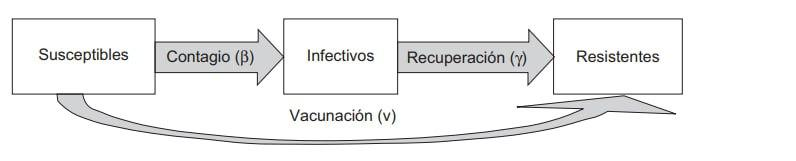
\includegraphics[width=1.0\textwidth,height=5cm]{Esquema1.jpg}
	\caption{Din\'amica epid\'emica de la enfermedad}
\end{figure}
\subsubsection{Ecuaciones}
Sistema de ecuaciones empleado:
\begin{equation}
\hspace{-7em}
\begin{aligned}
	\begin{pmatrix}
		S'\\
		I'\\
		R'\\
	\end{pmatrix}
	=
\begin{array}{l}
S'(x) = -\beta*I(t)*S(t)-V(t) \\
I'(x) = \beta*I(t)*S(t)- \gamma*I(t); \ siendo \ N = S(t)+I(t)+R(t)\\
R'(x) = \gamma*I(t)+ V(t)
\end{array}
\end{aligned}
\end{equation}

\begin{equation}
\hspace{-28em}
V(t)=
\begin{aligned}
\left\{
\begin{array}{l}
	0 \ si\  0 \le t \le 9 \\
	V \ si\  9 < t \le 18 \\
	0 \ si\  18 < t \le 51 \\
\end{array}
\right.
\end{aligned}
\end{equation}

\subsection{Linealizaci\'on y Estabilidad}
El sistema $(1)$ al tratar de ser resuelto para el vector soluci\'on nulo arroja como condici\'on necesaria y suficiente
que la funci\'on I(t) sea nula y que $t>19$.\\\\

Por otra parte la matriz jacobiana del sistema viene dada por la expresi\'on:\\
\begin{aligned}
\begin{pmatrix}
$f_S(S_0,I_0,R_0)$ & $f_I(S_0,I_0,R_0)$ & $f_R(S_0,I_0,R_0)$\\

$g_S(S_0,I_0,R_0)$ & $g_I(S_0,I_0,R_0)$ & $g_R(S_0,I_0,R_0)$\\

$h_S(S_0,I_0,R_0)$ & $h_I(S_0,I_0,R_0)$ & $h_R(S_0,I_0,R_0)$\\
\end{pmatrix}
\end{aligned}\\
Y sus valores son:\\\\
\begin{aligned}
	\begin{pmatrix}
	$0$ & $3.05$ & $0$\\
	
	$0$ & $-0.41$ & $0$\\
	
	$0$ & $3.47$ & $0$\\
	\end{pmatrix}
	\end{aligned}\\\\

Esta matriz se convierte en una matriz de coeficientes para el sistema linealizado
$X'=J*x$ donde $X'$ es el vector compuesto por las funciones $u_1', u_2', u_3'$ tal que 
$u_1 = S(t)- S_0$, $u_2 = I(t)-I_0$ y $u_3 = R(t)- R_0$, $X$ es la transpuesta del vector compuesto por 
las funciones $u_1, u_2, u_3$ y el punto $(S_0,I_0,R_0)$ es el punto de equilibrio analizado.\\

Los valores propios del Jacobiano evaluados en el punto de equilibrio son: 0, 0 y -0.4171
por lo cual podemos concluir que el punto de equilibrio en cuesti\'on es un nodo estable ya que
los ceros no aportan informaci\'on y al ser el resto de los valores, en este caso uno, negativos
se confirma la estabilidad de dicho nodo.

\subsection[short]{M\'etodos y algoritmos utilizados}
Para corroborar los resultados mostrados en este paper, se demostro la estabilidad
del sistema, se recrearon los diagramas de fase y
se us\'o el m\'etodo de Runge-Kutta de 4to orden (RK4)
teniendo en cuenta la tabla de valores iniciales(Cuadro 1).
\begin{table}[htbp]
	\centering
	\caption{Valores iniciales usados en la simulación}
	\label{tabla-ejemplo}
	\begin{tabular}{|c|c|c|}
		\hline
		\textbf{Párametro} & \textbf{Valor} \\
		\hline
		\'Indice per c\'apita de cobertura vacunal, & 0,20 \\
		N\'umero total de individuos & 100'000\\
		Coeficiente de transmisi\'on($\beta$) & $ 3.614\times10^-5$\\
		Coeficiente de retiro natural($\gamma$) & 3.47\\
		\'Indice per c\'apita de eficacia de la vacuna & 0.67\\
		Susceptibles iniciales &99'986\\
		Infectivos iniciales & 14\\
		Resistentes iniciales & 0\\
		Semanas de estudio epidm. & 52\\
		\hline
	\end{tabular}
\end{table}
\\
\clearpage

\begin{figure}
	\section*{Gr\'aficos}\\

	\centering
	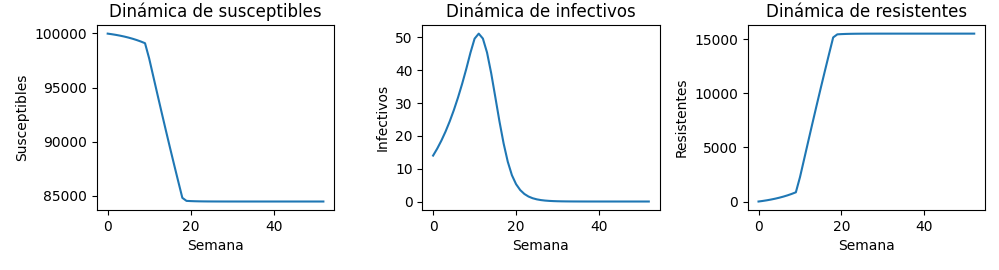
\includegraphics[width=1.0\textwidth,height=5cm]{Figure_1.png}
	\caption{Gráficas en función del tiempo si se realiza la vacunación}
	\centering
	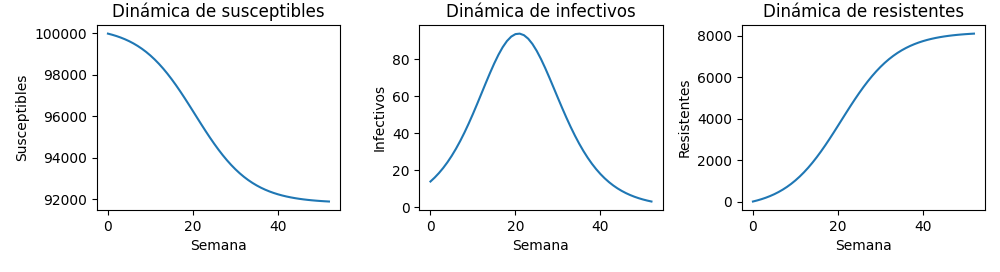
\includegraphics[width=1.0\textwidth,height=5cm]{Figure_2.png}
	\caption{Gráficas en función del tiempo si no se realiza la vacunación}\centering
	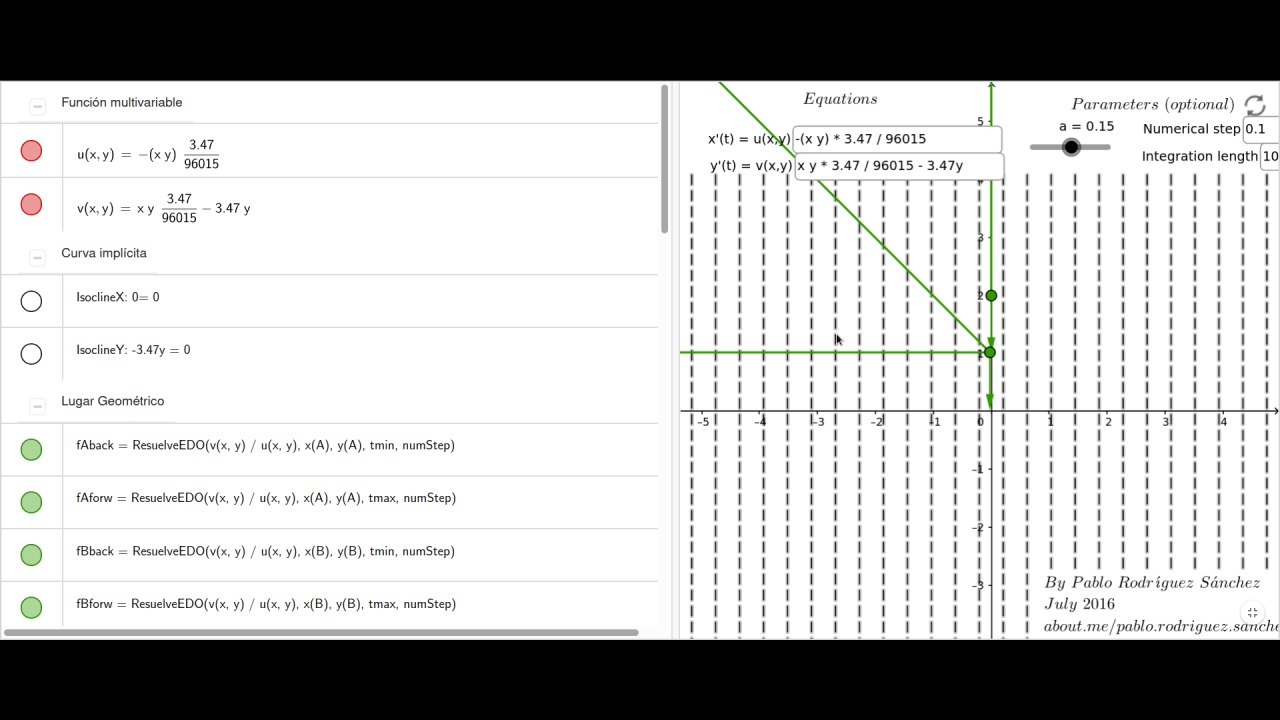
\includegraphics[width=1.0\textwidth,height=5cm]{fig3.jpg}
	\caption{Diagrama de Fases }

\end{figure}

\section*{REFERENCIAS}
https://www.gacetasanitaria.org/es-uno-coma-uno-siete-dos-tenemos-factor-articulo-S0213911110001743
https://www.gacetasanitaria.org/es-gaceta-sanitaria-2022-maximo-factor-articulo-S0213911123000092
Ecuaciones Diferenciales y problemas con valores en la Frontera. C/'omputo y Modelado. Cuarta Edici/'on. Aut: C. Henry Edwards, David E. Penney

\appendix

\clearpage
\section{Anexos} \label{app:quadratic}
\begin{lstlisting}[language=python]
	def tamanno_poblacion <- 100000;
	def susceptibles <- 99986;
	def infectivos <- 14;
	def resistentes <- 0;
	def susceptibles_auge_onda_epidemica <- 96015;
	def coeficiente_retiro_natural <- 3.47;
	def eficacia_vacuna: float <- 0.67;
	def cobertura_vacunal: float <- 0.20;
	def coeficiente_transmision <- coeficiente_retiro_natural
		                     /susceptibles_auge_onda_epidemica;
	
	funcion edo(t, valores):
	 	(dx, dy, dz) <- valores;
		dxdt <- -coeficiente_transmision*dy*dx-Vacunados(t);
		dydt <- coeficiente_transmision*dy*dx
			   -coeficiente_retiro_natural*dy;
		dzdt <- coeficiente_retiro_natural*dy+Vacunados(t);
		retorna Arreglo(dxdt, dydt, dzdt);
	
	funcion Vacunados(tiempo):
		Si tiempo >= 0 y tiempo <= 9 Entonces
			retorna 0
		Si tiempo > 9 y tiempo <= 18 Entonces
			retorna tamanno_poblacion*eficacia_vacuna*
					cobertura_vacunal/9.0
		Si tiempo>18 Entonces
			retorna 0
	
	funcion runge_kutta4(f, x0, y0, h, n):
		ArregloSoluciones <- [(x0, y0)]
		Desde i=1 hasta n Hacer
			(xi, yi) <- ArregloSoluciones.UltimoElemento
			k1 <- h * f(xi, yi)
			k2 <- h * f(xi + h/2, yi + k1/2)
			k3 <- h * f(xi + h/2, yi + k2/2)
			k4 <- h * f(xi + h, yi + k3)
			y_next <- yi + (k1 + 2*k2 + 2*k3 + k4)/6
			x_next <- xi + h
			ArregloSoluciones.Annadir((x_next, y_next))
		Siguiente	

		retorna ArregloSoluciones

	Resultados = runge_kutta4(edo, 0, [99986, 14, 0], 1, 52)

\end{lstlisting}


\end{document}

